\documentclass[a4paper,11pt]{jarticle}

% レイアウト
\setlength{\hoffset}{0cm}
\setlength{\oddsidemargin}{-3mm}
\setlength{\evensidemargin}{-3cm}
\setlength{\marginparsep}{0cm}
\setlength{\marginparwidth}{0cm}
\setlength{\textheight}{24.7cm}
\setlength{\textwidth}{17cm}
\setlength{\topmargin}{-45pt}


\renewcommand{\baselinestretch}{1.2}
\renewcommand{\floatpagefraction}{1}
\renewcommand{\topfraction}{1}
\renewcommand{\bottomfraction}{1}
\renewcommand{\textfraction}{0}
\renewcommand\thefootnote{\arabic{footnote})}

% パッケージ
\usepackage[dvipdfmx]{graphicx}
\usepackage{amsmath,amssymb,epsfig}
\usepackage{eucal}
\usepackage{bm}
\usepackage{ascmac}
\usepackage{pifont}
\usepackage{multirow}
\usepackage{enumerate}
\usepackage{cases}
\usepackage{type1cm}
\usepackage{cancel}
\usepackage{url}
\usepackage{cite}
%\usepackage{color}
\usepackage[dvipdfmx]{color}
\usepackage{caption}
\usepackage[caption=false]{subfig}
\captionsetup[figure]{labelsep=space}
\usepackage{here}

% 擬似コード作成用
\usepackage[ruled,vlined]{algorithm2e}
\usepackage{setspace}
\DeclareRelationFont{JY1}{mc}{it}{}{OT1}{cmr}{it}{}
\DeclareRelationFont{JT1}{mc}{it}{}{OT1}{cmr}{it}{}
\DeclareFontShape{JY1}{mc}{m}{it}{<5> <6> <7> <8> <9> <10> sgen*min
    <10.95><12><14.4><17.28><20.74><24.88> min10
    <-> min10}{}
\DeclareFontShape{JT1}{mc}{m}{it}{<5> <6> <7> <8> <9> <10> sgen*tmin
    <10.95><12><14.4><17.28><20.74><24.88> tmin10
    <-> tmin10}{}
\DeclareRelationFont{JY1}{mc}{sl}{}{OT1}{cmr}{sl}{}
\DeclareRelationFont{JT1}{mc}{sl}{}{OT1}{cmr}{sl}{}
\DeclareFontShape{JY1}{mc}{m}{sl}{<5> <6> <7> <8> <9> <10> sgen*min
    <10.95><12><14.4><17.28><20.74><24.88> min10
    <-> min10}{}
\DeclareFontShape{JT1}{mc}{m}{sl}{<5> <6> <7> <8> <9> <10> sgen*tmin
    <10.95><12><14.4><17.28><20.74><24.88> tmin10
    <-> tmin10}{}
\DeclareRelationFont{JY1}{mc}{sc}{}{OT1}{cmr}{sc}{}
\DeclareRelationFont{JT1}{mc}{sc}{}{OT1}{cmr}{sc}{}
\DeclareFontShape{JY1}{mc}{m}{sc}{<5> <6> <7> <8> <9> <10> sgen*min
    <10.95><12><14.4><17.28><20.74><24.88> min10
    <-> min10}{}
\DeclareFontShape{JT1}{mc}{m}{sc}{<5> <6> <7> <8> <9> <10> sgen*tmin
    <10.95><12><14.4><17.28><20.74><24.88> tmin10
    <-> tmin10}{}
\DeclareRelationFont{JY1}{gt}{it}{}{OT1}{cmbx}{it}{}
\DeclareRelationFont{JT1}{gt}{it}{}{OT1}{cmbx}{it}{}
\DeclareFontShape{JY1}{mc}{bx}{it}{<5> <6> <7> <8> <9> <10> sgen*goth
    <10.95><12><14.4><17.28><20.74><24.88> goth10
    <-> goth10}{}
\DeclareFontShape{JT1}{mc}{bx}{it}{<5> <6> <7> <8> <9> <10> sgen*tgoth
    <10.95><12><14.4><17.28><20.74><24.88> tgoth10
    <-> tgoth10}{}
\DeclareRelationFont{JY1}{gt}{sl}{}{OT1}{cmbx}{sl}{}
\DeclareRelationFont{JT1}{gt}{sl}{}{OT1}{cmbx}{sl}{}
\DeclareFontShape{JY1}{mc}{bx}{sl}{<5> <6> <7> <8> <9> <10> sgen*goth
    <10.95><12><14.4><17.28><20.74><24.88> goth10
    <-> goth10}{}
\DeclareFontShape{JT1}{mc}{bx}{sl}{<5> <6> <7> <8> <9> <10> sgen*tgoth
    <10.95><12><14.4><17.28><20.74><24.88> tgoth10
    <-> tgoth10}{}
\DeclareRelationFont{JY1}{gt}{sc}{}{OT1}{cmbx}{sc}{}
\DeclareRelationFont{JT1}{gt}{sc}{}{OT1}{cmbx}{sc}{}
\DeclareFontShape{JY1}{mc}{bx}{sc}{<5> <6> <7> <8> <9> <10> sgen*goth
    <10.95><12><14.4><17.28><20.74><24.88> goth10
    <-> goth10}{}
\DeclareFontShape{JT1}{mc}{bx}{sc}{<5> <6> <7> <8> <9> <10> sgen*tgoth
    <10.95><12><14.4><17.28><20.74><24.88> tgoth10
    <-> tgoth10}{}
\DeclareRelationFont{JY1}{gt}{it}{}{OT1}{cmr}{it}{}
\DeclareRelationFont{JT1}{gt}{it}{}{OT1}{cmr}{it}{}
\DeclareFontShape{JY1}{gt}{m}{it}{<5> <6> <7> <8> <9> <10> sgen*goth
    <10.95><12><14.4><17.28><20.74><24.88> goth10
    <-> goth10}{}
\DeclareFontShape{JT1}{gt}{m}{it}{<5> <6> <7> <8> <9> <10> sgen*tgoth
    <10.95><12><14.4><17.28><20.74><24.88> tgoth10
    <-> tgoth10}{}
\endinput
%%%% end of jdummy.def

% カウンタの設定
\setcounter{section}{0}
\setcounter{subsection}{0}
\setcounter{subsubsection}{0}
\setcounter{equation}{0}

% キャプションの図をFigに変更
\renewcommand{\figurename}{Fig.}
\renewcommand{\tablename}{Tab.}

% 式番号を式(章番号.番号)に
\makeatletter
\renewcommand{\theequation}{\arabic{equation}}
\@addtoreset{equation}{section}
\makeatother

% タイトル部分
\title{\vspace{-20truemm}
{\normalsize \rightline{平成29年\ 10月\ 25日}}
{\large 確率システム制御特論\\}
第4回演習問題\\
\date{}
\vspace{-2truemm}}
\author{機械知能工学専攻 知能制御工学コース \hspace{3mm} 17344219 \ 二宮 悠二}
%---------------------------------------------
% ドキュメントの開始
\begin{document}
\parindent = 0pt % 字下げoff
% 表紙
\titlepage
\maketitle
%---------------------------------------------
% 課題内容
{\Large{\bf 問題}}
%---------------------------------------------
\begin{enumerate}
 \item ベイズの定理の証明をせよ.
%-----------------------------------
 \item $ x_1, x_2, \cdots , x_N $が平均$ \mu $,分散$ \sigma^2 $の正規分布から独立に発生した数値データであるとき,これらの平均値$ \bar{\mu} $,分散$ \bar{\sigma}^2 $の最尤推定量を求めよ(解答例中の数式$ \textcircled{\scriptsize 1} 〜 \textcircled{\scriptsize 6} $を記述せよ).
\end{enumerate}
%-----------------------------------
%---------------------------------------------
{\Large{\bf 解答}}
%---------------------------------------------
\begin{enumerate}
 \item 
\ \ ベイズの定理とは,次式で与えられる条件付き確率に関して成り立つ定理である.
%-----------------------------------
\begin{equation}
 P(A|B) = \dfrac{P(A)P(B|A)}{P(A)}
\end{equation}
%-----------------------------------
この定理が成り立つことを証明する.\\\\
(証明)\\
\ \ ある標本空間で定義される二つの事象$ A,B $について,次のような三つの確率が定義できる.
%-----------------------------------
\begin{itemize}
 \item {\bf 同時確率}$ P(A,B) $:$ AとB $が同時に起こる確率.
 \item {\bf 周辺確率}$ P(A),P(B) $:他の事象に関わりのない一つの事象だけの確率
 \item {\bf 条件付確率}$ P(A|B) $:$B$が起きたという条件の元で$A$が起こる確率.
\end{itemize}
%-----------------------------------
上記の定義を用いて,条件付確率は次のように定義される.
%-----------------------------------
\begin{equation}
 P(A|B) = \dfrac{P(A,B)}{P(B)},~~ P(B|A) = \dfrac{P(A,B)}{P(A)}
\end{equation}
%-----------------------------------
このとき,$ P(A) \neq 0 $,$ P(B) \neq 0 $である.(2)式をそれぞれ変形すると,次式を得る.
%-----------------------------------
\begin{eqnarray}
 && P(A,B) = P(A|B)P(B) \\
 && P(A,B) = P(B|A)P(A)
\end{eqnarray}
%-----------------------------------
(3),(4)式は等しいので,次の関係式を得ることができる.
%-----------------------------------
\begin{eqnarray}
 P(A|B)P(B) & = & P(B|A)P(A) \nonumber \\
 P(A|B) & = & \dfrac{P(A)P(B|A)}{P(B)}
\end{eqnarray}
%-----------------------------------
\begin{flushright}
 (以上)
\end{flushright}
%\ \ $ m $個の事象$ A_1, ~ \ldots ~ , A_m $と$ n $個の事象$ B_1, ~ \ldots ~ , B_n $に対する同時確率$ P(A_m,B_n) $と周辺確率$ P(A_m)およびP(B_n) $
%-----------------------------------
%---------------------------------------------
 \item
\ \ まず,平均$ \mu $,分散$ \sigma^2 $の正規分布の確率密度は以下のように表せる.
%-----------------------------------
\begin{equation}
 p(x) = \dfrac{1}{\sqrt{2 \pi \sigma^2}} e^{-(x - \mu)^2 / 2 \sigma^2}
\end{equation}
%-----------------------------------
これより,尤度は次のように書ける.
%-----------------------------------
\begin{equation}
 L = \prod^N_{\alpha = 1} \textcircled{\scriptsize 1} = \textcircled{\scriptsize 2}
\end{equation}
%-----------------------------------
\begin{eqnarray*}
 & \textcircled{\scriptsize 1} & \dfrac{1}{\sqrt{2\pi\sigma^2}}e^{-(x_{\alpha}-\mu)^2/2\sigma^2} \\
 & \textcircled{\scriptsize 2} & \dfrac{1}{(\sqrt{2\pi\sigma^2})^N} \prod^N_{\alpha = 1} e^{-(x_{\alpha}-\mu)^2/2\sigma^2}
\end{eqnarray*}
%-----------------------------------
これを最大化する$ \mu $と$ \sigma^2 $を求めるためには,次の$ J = - {\rm log} L $を最小にする$ \mu $と$ \sigma^2 $を求めればよい.
%-----------------------------------
\begin{equation}
 J = \dfrac{1}{2 \sigma^2} \sum^N_{\alpha = 1} \textcircled{\scriptsize 3} + \dfrac{N}{2} {\rm log} 2 \pi \sigma^2
\end{equation}
%-----------------------------------
\begin{eqnarray*}
 & \textcircled{\scriptsize 3} & (x_{\alpha}-\mu)^2
\end{eqnarray*}
%-----------------------------------
これを$ \mu $と$ \sigma^2 $で微分して$ 0 $とおくと,それぞれ次のようになる.
%-----------------------------------
\begin{eqnarray}
 && \dfrac{ \partial J}{ \partial {\rm u } } = - \dfrac{1}{\sigma^2} \sum^N_{\alpha = 1} \left( x_{\alpha} - \mu \right) = 0 \\
 && \dfrac{ \partial J}{ \partial \sigma^2 } = \textcircled{\scriptsize 4} = 0
\end{eqnarray}
%-----------------------------------
\begin{eqnarray*}
 & \textcircled{\scriptsize 4} & -\dfrac{1}{2\sigma^4} \sum^N_{\alpha=1} (x_{\alpha}-\mu)^2 + \dfrac{N}{2\sigma^2}
\end{eqnarray*}
%-----------------------------------
これを$ \mu $と$ \sigma^2 $について解いたものを$ \bar{\mu} $と$ \bar{\sigma^2} $とすると,次のようになる.
%-----------------------------------
\begin{eqnarray}
 \bar{\mu} & = & \textcircled{\scriptsize 5} \\
 \bar{\sigma}^2 & = & \textcircled{\scriptsize 6}
\end{eqnarray}
%-----------------------------------
\begin{eqnarray*}
 & \textcircled{\scriptsize 5} & \dfrac{1}{N} \sum^N_{\alpha=1} x_{\alpha} \\
 & \textcircled{\scriptsize 6} & \dfrac{1}{N} \sum^N_{\alpha=1} (x_{\alpha}-\mu)^2
\end{eqnarray*}
%-----------------------------------
これより,母平均$ \mu $,母分散$ \sigma^2 $の最尤推定量$ \bar{\mu} $と$ \bar{\sigma}^2 $は,それぞれサンプル平均とサンプル分散に等しいことがわかる.
\end{enumerate}
% % 図の挿入

% \begin{figure}[b]
%  \begin{center}
%   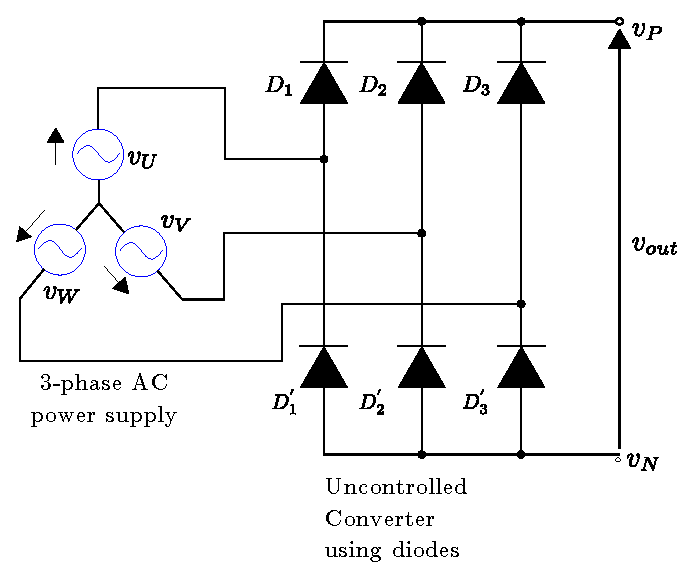
\includegraphics[scale=0.9]{../figure/circuit.eps}
%   \caption{Uncontrolled converter}
%   \label{circuit}
%  \end{center}
% \end{figure}


% % 表の挿入

% \begin{table}[htb]
%   \begin{center}
%     \caption{各素子のパラメータ}
%     \begin{tabular}{c|c|c} \hline
%       定数名[単位] & 記号 & 値 \\ \hline \hline
%       周波数[Hz] & $f_U,f_V,f_W$ & 120 \\ \hline
%                      & $\phi_U$ & $\frac{2\pi}{3}$ \\
%       初期位相角[rad] & $\phi_V$ & $\frac{4\pi}{3}$ \\
%                      & $\phi_W$ & $2\pi$ \\ \hline
%       抵抗[$\Omega$] & $R$ & 10 \\ \hline
%     \end{tabular}
%     \label{param}
%   \end{center}
% \end{table}


% % 図の挿入

% \begin{figure}[tb]
%  \centering
%  \vspace{0.5cm}
%  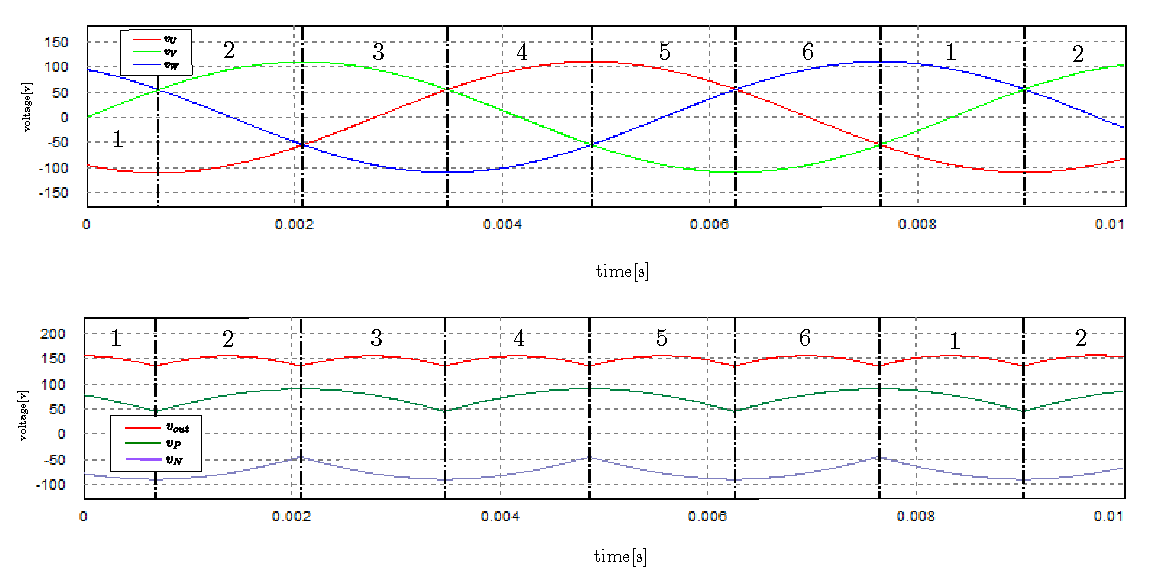
\includegraphics[scale=0.85]{../figure/waves.eps}\\
%  \hspace{0.0cm}
%  % 入力と出力\\
%  % \\
%  % \vspace{1.2cm}
%  % 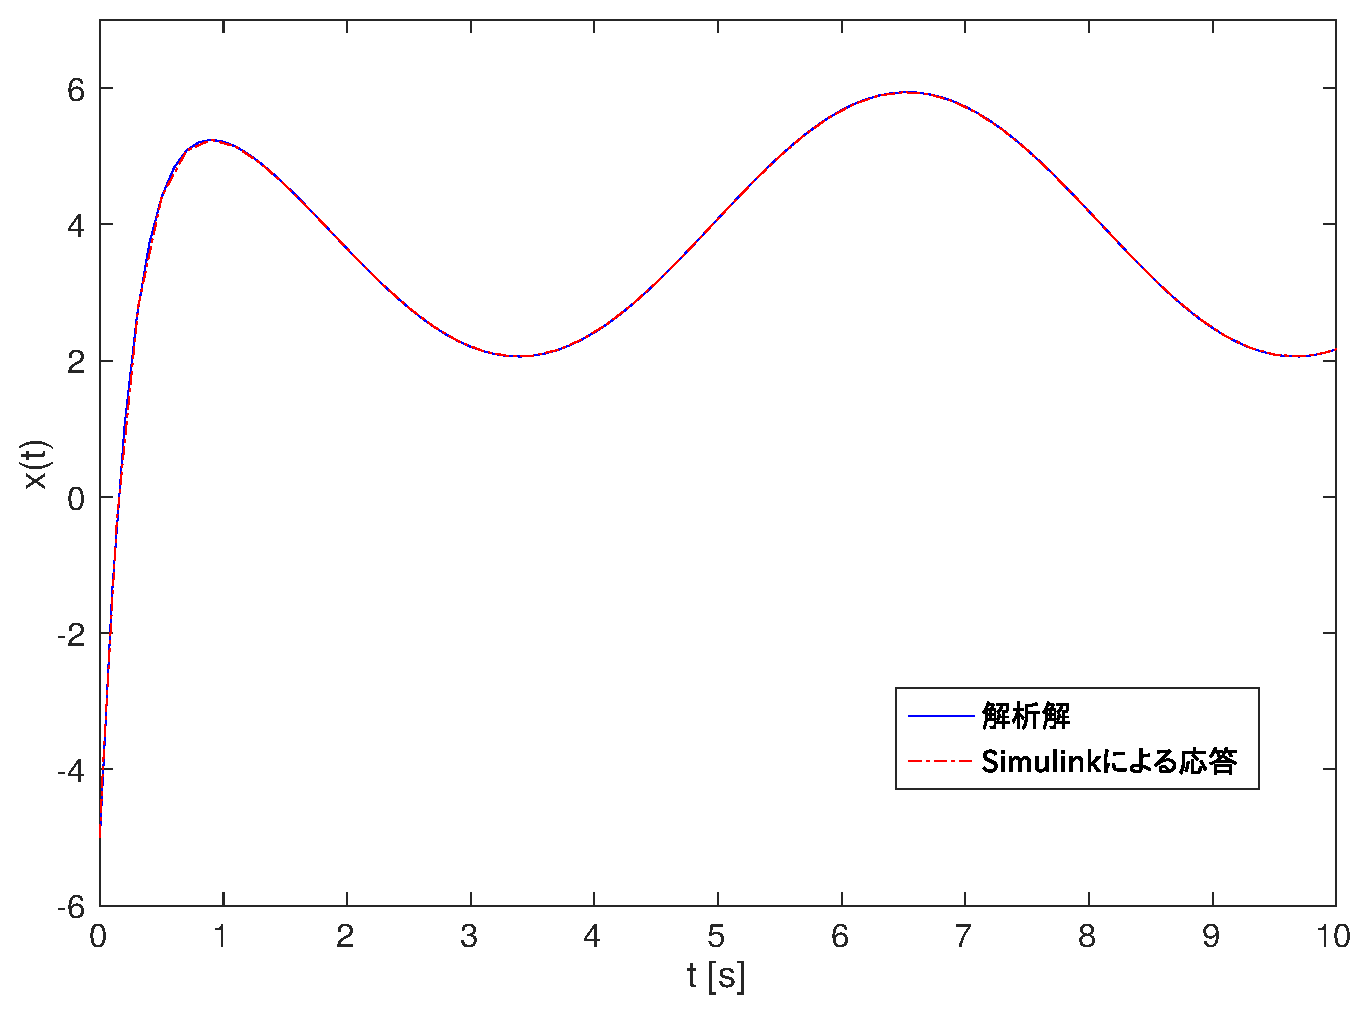
\includegraphics[scale=0.825]{../figure/output.eps}\\
%  % (b) 出力の電位\\
%  % \\
%  \caption{シミュレーションにより得られた各電源電圧(上)と出力電位(下)の波形}
%  \label{wave}
% \end{figure}

% \newpage

% % 図を並べて挿入

% \begin{figure}[tb]
%  \centering
%  \subfloat[区間1における回路動作]{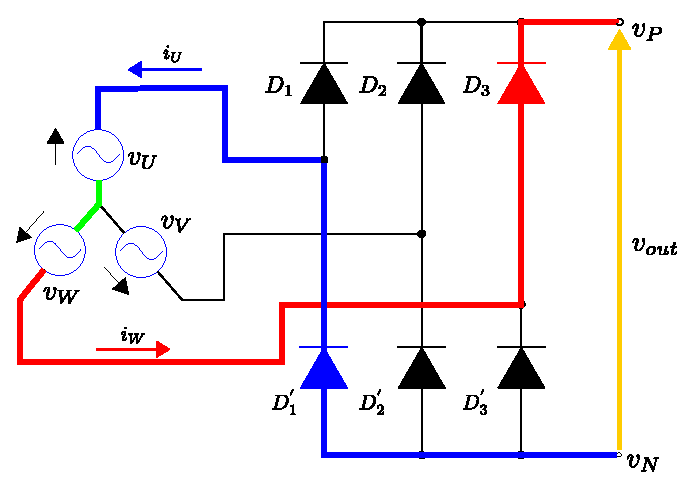
\includegraphics[scale=0.5]{../figure/kukan_1.eps}}
%  \hspace{1.5cm}
%  \subfloat[区間2における回路動作]{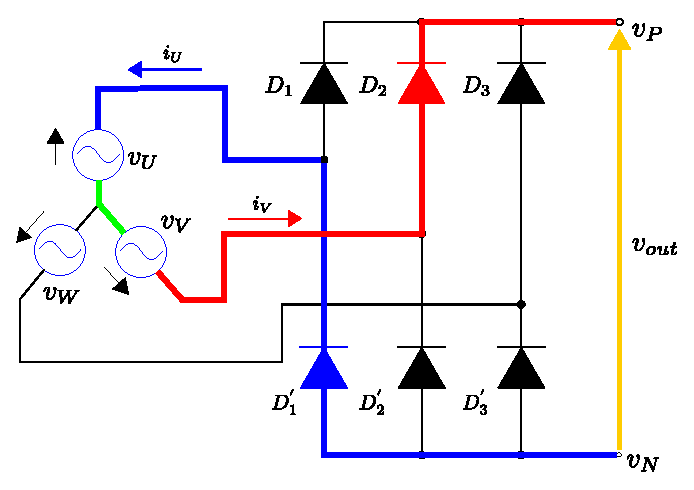
\includegraphics[scale=0.5]{../figure/kukan_2.eps}}
% \\
%  \vspace{0.5cm}
%  \subfloat[区間3における回路動作]{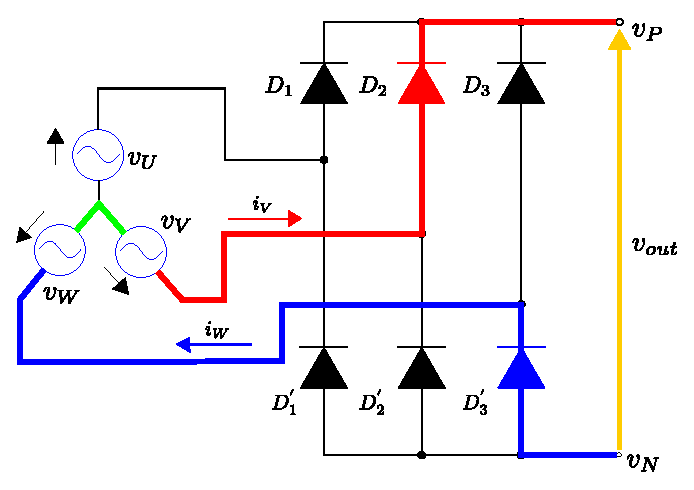
\includegraphics[scale=0.5]{../figure/kukan_3.eps}}
%  \hspace{1.5cm}
%  \subfloat[区間4における回路動作]{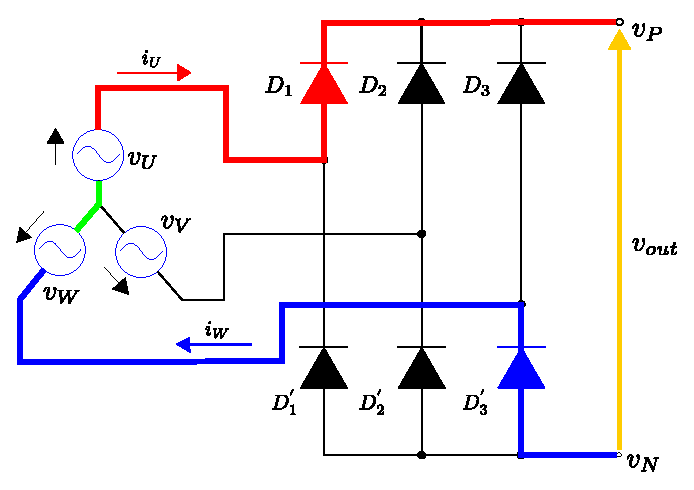
\includegraphics[scale=0.5]{../figure/kukan_4.eps}}
% \\
%  \vspace{0.5cm}
%  \subfloat[区間5における回路動作]{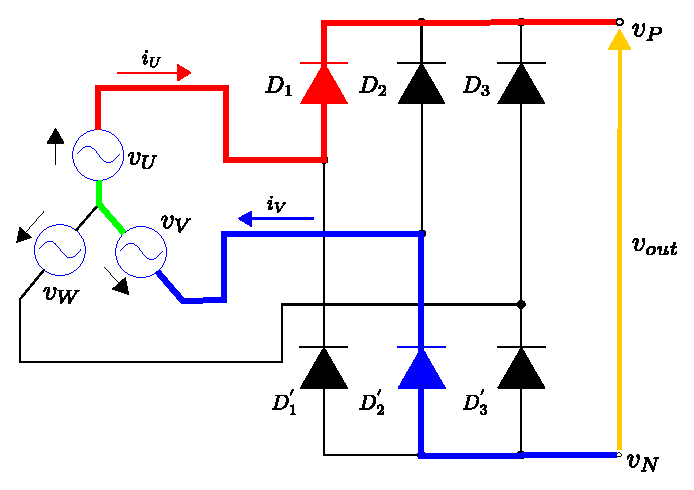
\includegraphics[scale=0.5]{../figure/kukan_5.eps}}
%  \hspace{1.5cm}
%  \subfloat[区間6における回路動作]{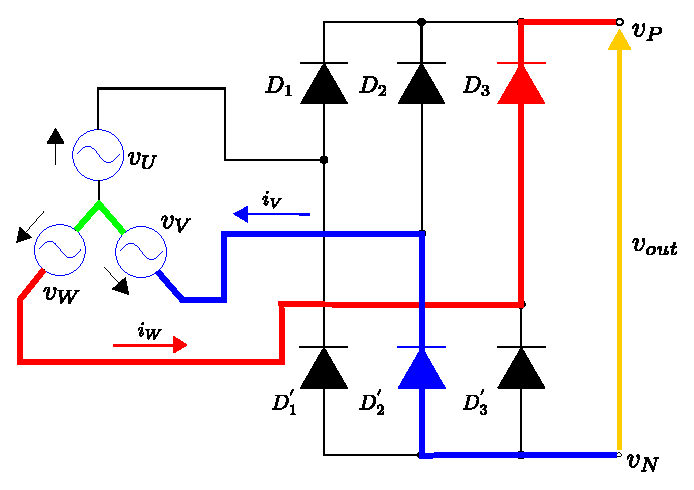
\includegraphics[scale=0.5]{../figure/kukan_6.eps}}
% \\
%  \caption{各区間での回路動作の様子}
%  \label{circuit_kaku}
% \end{figure}

% % 文中へのラベリング
% {\bf Fig. }\ref{circuit_kaku}に示す〜

% 参考文献
\begin{thebibliography}{99}
\addcontentsline{toc}{section}{参考文献}
\bibitem{1} 足立 修一・丸田 一郎,”カルマンフィルタの基礎”,東京電機大学出版局,pp.76-80,2012.
%\bibitem{data} UCI Machine Learning Repositiry,SECOM Data Set,https://archive.ics.uci.edu/ml/datasets/SECOM,(最終閲覧日:2017年10月18日).
\end{thebibliography}

\end{document}
